

\chapter{轻轻松松学统计分析} % Introduction chapter suppressed from the table of contents


小李刚中学毕业,希望去工厂找工作。\\
问:工厂员工薪水是多少?\\
人事部经理面带笑容地跟他说:我们工厂员工平均月收入大概3300。\\
小李进了工厂后,才发现绝大部分的工人月薪是2000;
有多年经验的工人可以拿到2400。但他们有少数的管理层,他们的平均月薪是25,000。



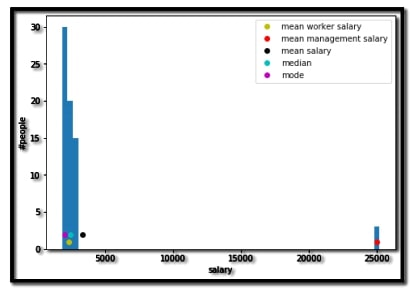
\includegraphics[width=10cm]{AverageSalaryScreenshot_2021-07-31_171502.jpg}

所以人事部经理没有``骗''小李,工厂员工平均收入是每月3309。

其实我们天天在媒体/广告都看到利用统计分析来误导的例子,所以Darrell HUFF
先生在1954年写了《How to Lie with
Statistics》,专门描述如何利用统计撒谎。

如果你觉得统计学很高深,避而远之,你可以看看这上下两篇如何教小孩统计分析的故事。

估计当你再看到下面这类统计结果,你会有新的想法:

\framebox{%
\begin{minipage}[t]{0.97\columnwidth}\raggedright
\vtop{\hbox{\strut 我们读者年龄的中位数是34岁,平均的家庭年收入是7270美元。}\hbox{\strut :::``时代杂志''
主编}}\tabularnewline
\strut
\end{minipage}}

\hypertarget{ux4eceux8003ux8bd5ux6210ux7ee9ux5230ux8d38ux6613ux9006ux5dee}{%
\section{从考试成绩到贸易逆差}\label{ux4eceux8003ux8bd5ux6210ux7ee9ux5230ux8d38ux6613ux9006ux5dee}}

孩子问:爸爸,你是做什么工作的?我明天要在班上介绍自己父母的工作。\\
我说:帮客户做统计分析。\\
孩子问:统计分析?\\
我心里想你这初中孩子,要如何给你解释统计分析呢?\\
我尝试用一个他可以想象的场景来介绍------假如下面是你班里同学的数学成绩,你会用什么方式把这些成绩表达出来?\\
孩子有点迷茫。\\
=== 20名学生在数学考试中的分数(满分为100分,按大小排序) ===

30, 35, 37, 40, 40, 49, 51, 54, 54, 55\\
57, 58, 60, 60, 62, 62, 65, 67, 74, 89

我接着说:任何样本数据,都可以用图加平均值、范围等来表达。\\
举例:我们可以用茎叶图(Stem and leaf
plot){[}详见附件A1{]}表达这些学生成绩:\\

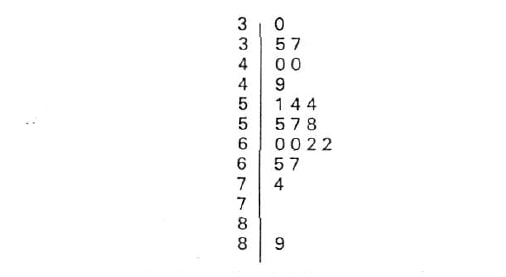
\includegraphics[width=10cm]{MA_FA2_1_0.jpg}\\
把20组数,从最低排到最高。 排在第十位学生和第十一位学生的平均数
56,叫中位数(Median)。 排第五名和第六名成绩的平均值 44.5,就是 Q1
四分之一。 排十五名和十六名的平均值 62,就是 Q3 四分之三。

这个茎叶图,再加上Q1 ,中位数(Q2),Q3 ,{[}44.5 , 56 , 62{]}
便可以总括表达这二十个学生的成绩分布。
也可以用下面的柱状图(Histogram)来表达:\\

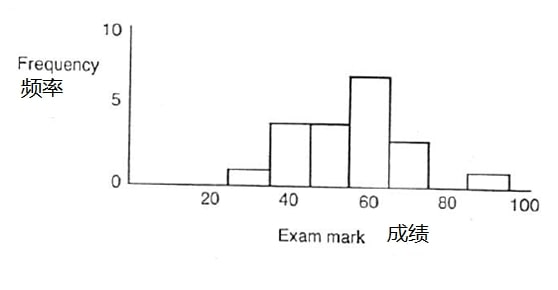
\includegraphics[width=10cm]{MA_FA1_1_0.jpg}\\

除了中位数,也常用平均值(Mean)来表示一堆数据的中间趋势,平均值就是把所有数据加起来,然后把总数除以数量,比如上面20学生数学成绩的平均值是......
孩子充满自信,打断我说:这个平均值简单,我懂。\\
我说:好啊,你这么懂平均值,我问你一个小问题:\\

5 , 10 , 350 ,
355的平均数是多少?\\

\textbar{}\}

孩子拿了计算器算出:180。\\
我说:你知道那些数是代表什么吗?\\
孩子说:不知道。\\
如果这些数是代表角的度数,它的平均值应该是零,而不是
180。这是统计分析很重要的概念 ------
你必须知道那些数的背景,否则你的分析没意义。如果你把那四个数字当成是距离来算均值是
180,与四个角度数求均值的结果就完全不一样了。\\
从以上例子,你就知道了解问题背景(Context)很重要。

孩子问:这些统计分析有什么用?\\
答:例如,有了这成绩的分析,你就可以知道自己的成绩在整个班是处于什么位置?也可以帮你比较不同科目的成绩。

\hypertarget{ux6bd4ux8f83ux4e09ux79cdux6559ux5b66ux65b9ux6cd5}{%
\subsubsection{比较三种教学方法}\label{ux6bd4ux8f83ux4e09ux79cdux6559ux5b66ux65b9ux6cd5}}

比较不同算术教学方法的实验中,45名学生被随机分成5个大小相同的组。两组(A,B)采用目前使用的方法(控制组),另外三组(C,D,E)采用三种新方法。实验结束时,所有学生参加了一次标准测试,结果(满分30分)见表B.1。关于教学方法的差异,可以得出什么结论?\\

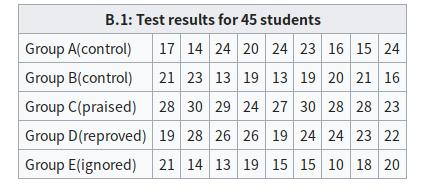
\includegraphics[width=10cm]{Screenshotfrom2022-01-18-2.jpg}


C (praised) = 赞赏, D(reproved)=责骂惩罚, E(ignored)=不理睬

我说:你可以用刚学过的东西汇总每一组数据,然后看看有没有差异。这样你便可以比较五个班的成绩。\\
他过了十五分钟就画了出来那个五个班的箱线图{[}详见附件A2{]}:\\

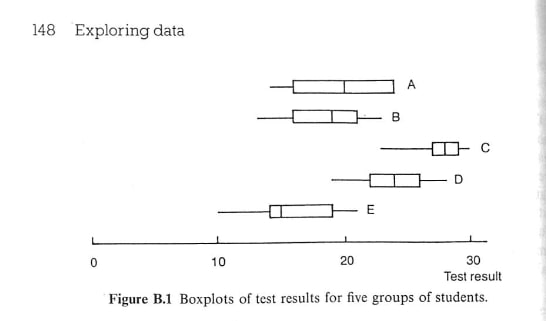
\includegraphics[width=10cm]{图片61-3.jpg}

我就问他:从这些图有看到显著区分嘛?\\
孩子答:看得出是C班最好,D班也比较好,E班就比较差。\\
我说:是的,但如果我们只是比较5个班成绩的平均值,没有考虑每一班成绩范围,便不能全面比较
-\/- 例如:上面数学考试成绩的Q1 Q2 Q3是 (44.5 , 56 , 62)
如果C班的数学成绩是(32 , 57.5 , 63)
你会认为C班比你们好吗?虽然中位数比你们班高,但Q1
比你们低很多,所以不能单看中位数(或平均值)比较。

看到他对这些挺有兴趣,我便问他如何表达以下数据:\\

\hypertarget{ux4ebaux4e00ux5e74ux5185ux9605ux8bfbux6708ux520aux7684ux6570ux91cf}{%
\subsubsection{20人一年内阅读月刊的数量}\label{ux4ebaux4e00ux5e74ux5185ux9605ux8bfbux6708ux520aux7684ux6570ux91cf}}

0, 1, 11, 0, 0, 0, 2, 12, 0, 0\\
12, 1, 0, 0, 0, 0, 12, 0, 11, 0

我看他开始使用同样方法,
我便说这些统计数据跟前面学生成绩的分布不一样,它一头一尾最高,这表示大部分人要么就是不看杂志,要么就是每个月都看,这种分布就不合适用刚才那些方法去表达,只能说它有两个高峰,或者叫众数(mode),再配上一个柱状图。如果我们用中位数或者这些数的平均值,或三分位数来表达的话,反而是误导读者,不能正确的表达那些数据的分布。\\

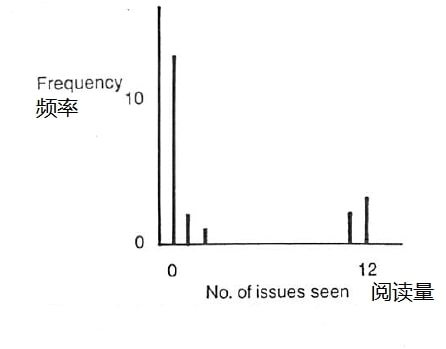
\includegraphics[width=10cm]{MA_FA4_1_0.jpg}\\
当总体(population)很大时,就只能抽样,用抽样来估计population分布。但是要注意,如果样本不是随机抽样(random
sample),可能会导致出来的参数偏离、有误差。\\
我看孩子一头雾水,但我记得他很喜欢研究二战的战斗机,我就用下面这个例子说明这样抽样出来的结论是没有意义。\\

\hypertarget{ux6837ux672cux504fux5dee-survivors-bias}{%
\subsubsection{样本偏差 Survivor's
Bias}\label{ux6837ux672cux504fux5dee-survivors-bias}}

错误的抽样会导致错误结论。

\framebox{%
\begin{minipage}[t]{0.97\columnwidth}\raggedright
二战时会对那些没有被击落的战斗机,研究哪个部分被德军的攻击最多,针对这些部位去加强防护,希望增高飞机的存活率。你同意吗?我们只是抽样了未被击落的飞机,被击落的都未被抽样。一个比较正确的抽样是所有两类都抽样才比较合理。\\
其实被击落的飞机哪个部分被击中更重要,但是我们无法得到那些抽样,只可以从没有被击落的飞机去看,这是抽样的错误。所以分析得出的结论没有意义。\\

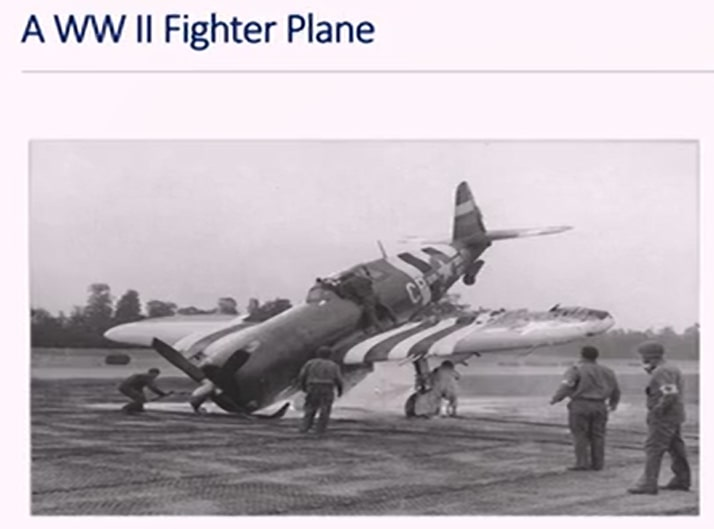
\includegraphics[width=10cm]{WW2Screenshot_2021-04-07_222054.jpg}
\strut
\end{minipage}}

孩子好像对统计越来越感兴趣。\\
我说:现在你开始知道什么叫统计了吗?明天可以跟老师讲故事了吗?\\
孩子追着问:可不可以再给我一个练习题?我觉得这统计学也没什么困难,我还可以把你给我的那些题目拿给我同桌小李试试,看他懂不懂。(男孩总是要当英雄,出风头)\\
我说:好啊。下面的身高统计数据,请你用刚才的方式来汇总一下,看看你学会没有?\\

\hypertarget{ux540dux5987ux5973ux53c2ux52a0ux67d0ux79cdux75beux75c5ux7814ux7a76ux5979ux4eecux7684ux8eabux9ad8ux4ee5ux7c73ux8ba1}{%
\subsubsection{20名妇女参加某种疾病研究,她们的身高(以米计)}\label{ux540dux5987ux5973ux53c2ux52a0ux67d0ux79cdux75beux75c5ux7814ux7a76ux5979ux4eecux7684ux8eabux9ad8ux4ee5ux7c73ux8ba1}}

1.52, 1.60, 1.57, 1.52, 1.60, 1.75, 1.73, 1.63, 1.55, 1.63\\
1.65, 1.55, 1.65, 1.60, 1.68, 2.50, 1.52, 1.65, 1.60, 1.65

他便拿着纸,用刚才学过的方式计算中位数、三分系数等。蛮有自信地画出图,交卷。\\
我就问他:你认识二点五米高的女性吗?\\
他说:真的好像没有。\\
所以里面那个2.5可能不对。你为什么没有疑问,直接去做?
统计分析必须要判断数据是否正确、靠谱。\\
统计学常常有一个说法叫``垃圾进,垃圾出 Garbage in, garbage
out'',如果数据本身不可靠,那么怎么分析都没用。\\
我接着说:也有很多人利用图表统计数据,误导读者。所以我们看一些统计专家的统计数据分析时也要小心。\\

\hypertarget{ux7f8eux56fdux4e2dux897fux90e8ux623fux4ef7ux8d8bux52bfux56fe}{%
\subsubsection{美国中西部房价趋势图}\label{ux7f8eux56fdux4e2dux897fux90e8ux623fux4ef7ux8d8bux52bfux56fe}}


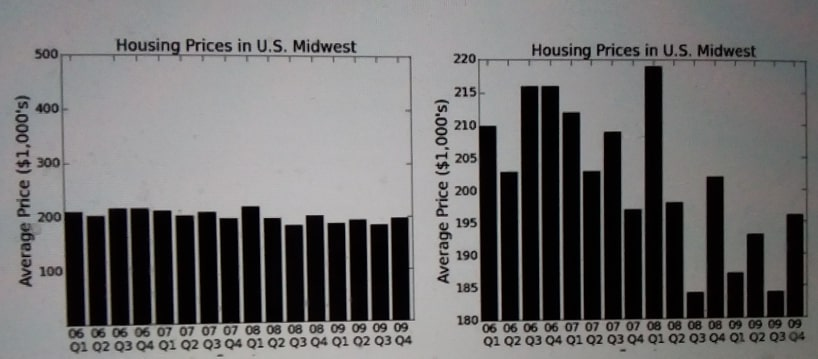
\includegraphics[width=10cm]{Stat_f22-1_1_1.jpg}

上图是06年到09年每个季度,美国中西部的房价。如果我们看右面那个柱状图,你会认为房价波动很大。但是如果同样这组数据看左面柱状图的话,你就会觉得没有太多变化。所以我们要注意人家用柱状图来表示的时候,要看左面坐标有没有标明数字。不应该仅仅看图。\\
虽然数据都一样,但如图形不一样,传达的信息便完全不同。\\
孩子说:你说这个我都懂啊,很简单嘛。\\
我看他这么有信心,我就问他:``你看这个来自报纸的统计图,你觉得有什么问题吗?''\\

\hypertarget{ux7f8eux56fdux5931ux4e1aux4ebaux6570-vs-ux5168ux804cux4ebaux6570}{%
\subsubsection{美国失业人数 vs
全职人数}\label{ux7f8eux56fdux5931ux4e1aux4ebaux6570-vs-ux5168ux804cux4ebaux6570}}


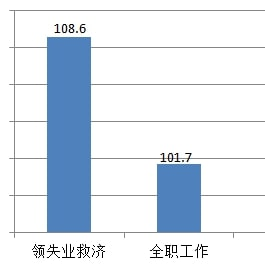
\includegraphics[width=10cm]{人数对比_2.jpg}

上图是美国接受失业救济金的人数与全职工作人数的对比,你是否会觉得失业人数比全职多很多?\\
如果你细看会发现Y坐标没有数量,也不是从零开始。看数据的话,左面比右面只多了6.8\%。

孩子说:你说的很有道理,如果按正常就不应该画出这个图,确实误导我们。\\
你可能会觉得失业人数比全职人数高还是很惊人。\\
我们细看它两边的数是怎么得出来:\\
左面失业救济金的人数的计算方法是:如果家庭其中一人接受救济金,全家的人数都计算在内。例如,一家单亲家庭母亲加4个孩子,母亲不是全职工作并收接受救济金,美国统计局会算5人接受失业救济金;另一家庭父母2人加3个孩子,只有父亲是全职工作,只算全职人数1位。

从以上例子,可以理解柱状图左右两数字不可以直接比较,好比不能因为A农夫年产20吨马铃薯,B年产3吨蓝莓,(假定农地大小相同)说A的生产率比B高同样道理。\\
\{\textbar{} class="wikitable" \textbar{}
另一个只挑选``合适的''来作比较的例子 (Picking cherries)\\

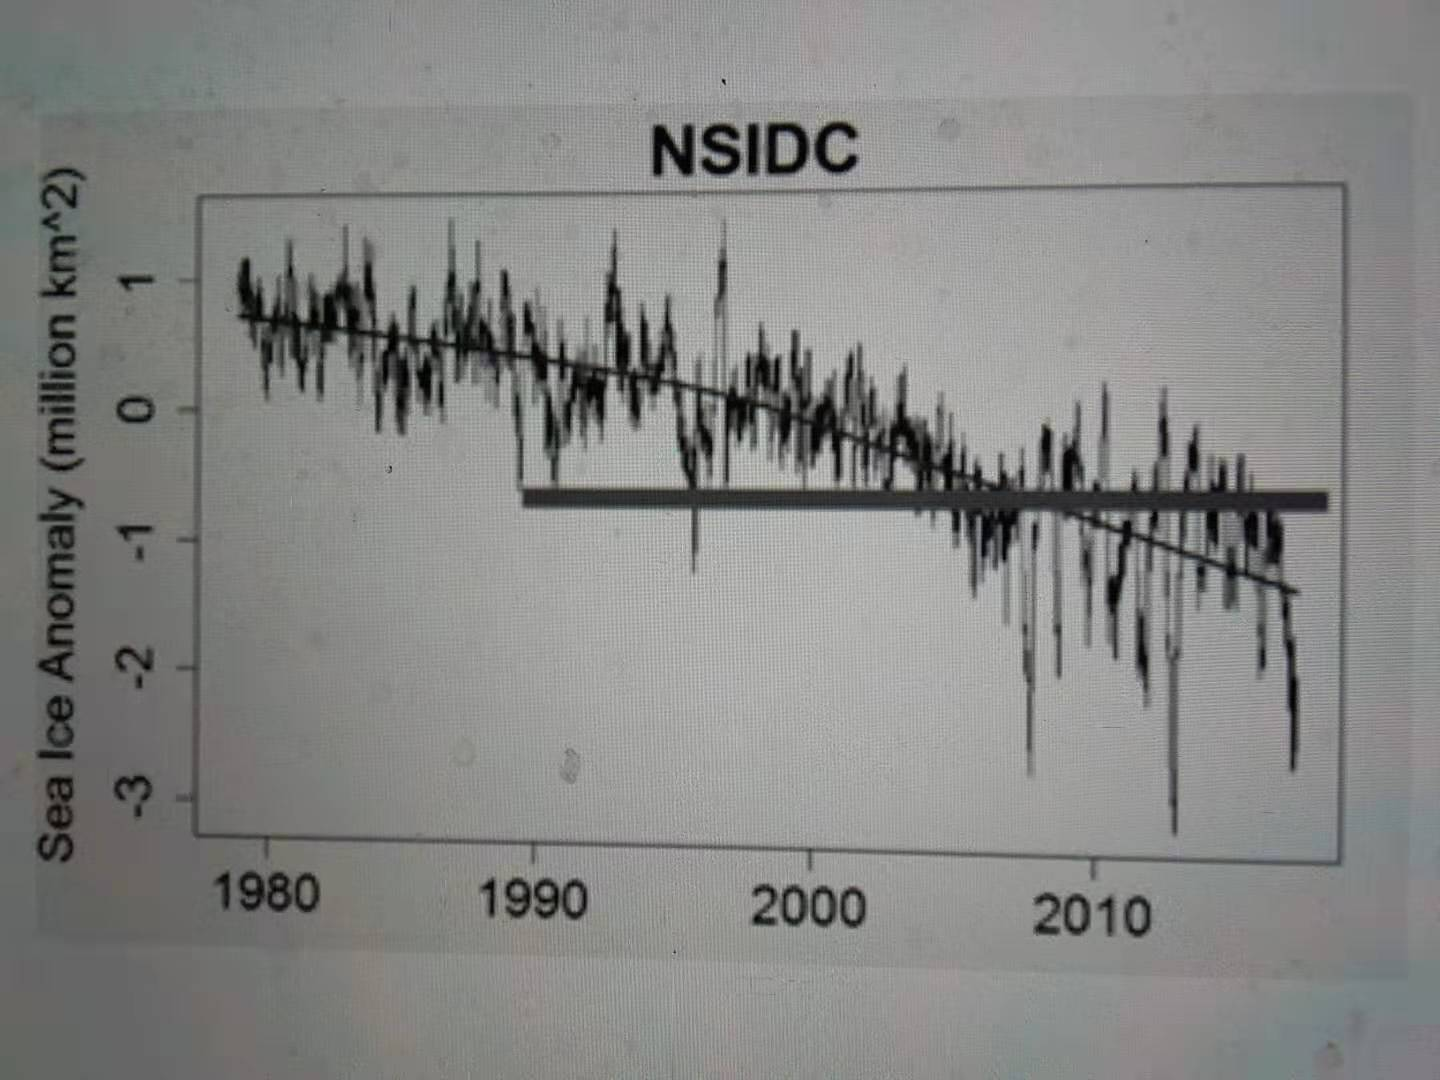
\includegraphics[width=10cm]{儿童MA.jpg}\\
*从上面八零年代到现在全球海洋冰量的统计很明显看到地球在不断地暖软化。但你还可以抽两个时间,例如:2012年四月份的冰量比1988年六月份多,来说明``全球变冷''!
\textbar{}\}

\hypertarget{ux5206ux6790ux4eceux8695ux8c46ux5b9eux9a8cux52306ux5e74ux9500ux552eux6570ux636e}{%
\section{分析:从蚕豆实验到6年销售数据}\label{ux5206ux6790ux4eceux8695ux8c46ux5b9eux9a8cux52306ux5e74ux9500ux552eux6570ux636e}}

第二天,孩子乖乖地来找我,他说:``爸爸,今天我跟老师说了你的工作是做统计分析,老师听到后就发给我一些高年级的生物实验数据,希望帮他做些分析,看看两类实验结果有没有差异。你可以帮忙吗?''\\

\hypertarget{ux8695ux8c46ux690dux7269-ux53ccux6837ux672ct-test}{%
\subsubsection{蚕豆植物-双样本t-test}\label{ux8695ux8c46ux690dux7269-ux53ccux6837ux672ct-test}}

以下数据显示了某一化学物质在蚕豆10个剪枝植株和10个生根植株中的(比例)浓度。\\
:剪枝: 53 58 48 18 55 42 50 47 51 45\\
:有根: 36 33 40 43 25 38 41 46 34 29\\
~\\
我说:你可以同样用昨天学过的方法(如,柱状图)比较两组数。\\
孩子就按这个汇总了两个实验数据的分布,如下图所示:\\

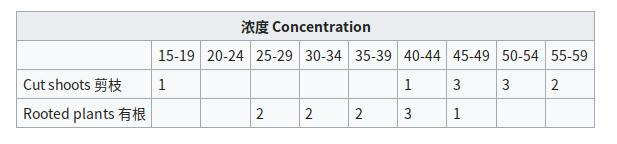
\includegraphics[width=10cm]{Screenshotfrom2022-01-18-3.jpg}

我看了一下,说:``这个你应该也看得懂:上面那个实验数据有一个很明显的异常点------18。你应该要问老师,这个18是错误数据还是一个值得相信的数?如果18是不对的,很明显地,你能发现第一个实验中的平均浓度比下面高\ldots{}\ldots{}''。当然,还有很多数据,并没有这么简单,我们就可以用一个叫``双样本t''的检验方式来比较两种数据是否有显著差异。但是如果有刚刚那种异常点,如直接用双样本
t
分析,因为第一组数据被那个18拉低了,结果很可能是两组没有显著差异。所以还是直接看数据的分布更实在。

我就给他总结一下:我们在统计学可以使用假设检验,其中包括双样本t检验比较,方差分析(ANOVA)等{[}详见附件A1,A2{]},就是针对这类统计数据分析。但是针对这个实验的数据,你从统计图一眼就能看出有显著区分,就不需要再采用这些假设检验方法,因为采用那些技巧不会得出额外的信息。\\
我接着跟他说:有些时候统计数据不是连续数据,像学生成绩、浓度、高度等,而是分组数据。例如下面这些国外人种眼睛颜色与头发颜色的数据,这种数据我们就需要用列联表
(Contingency Table) 来看这两个分组的变量之间有没有关系。\\

\hypertarget{ux5934ux53d1ux548cux773cux775bux989cux8272ux7684ux4e0dux540cux7ec4ux5408}{%
\subsubsection{头发和眼睛颜色的不同组合}\label{ux5934ux53d1ux548cux773cux775bux989cux8272ux7684ux4e0dux540cux7ec4ux5408}}

592人的头发和眼睛颜色的不同组合:

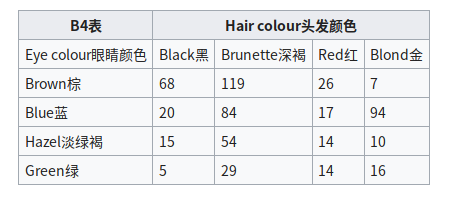
\includegraphics[width=10cm]{Screenshotfrom2022-01-18-4.jpg}



如果我们对上面 B4 表的数,加上每一行、每一列的总和,得出下面 B5
表,我们从每一列可看见,除了金发
(blond)那列例外,棕色(brown)眼睛的占大多(金发的大部分是蓝(blue)眼睛)。也看到金头发那列跟其他,如黑头发那列,分布不一样。比如我们看每行的话,也可以看到棕色眼睛跟蓝眼睛的数量差不多都是最多。但它们在金头发(blond)和黑头发(black)那列的分布就完全不同。统计分析的卡方检验{[}详见附件A3{]}也可以帮我们分析分组数据间有没有相关。但是像这类简单的4
X 4
数据表,只要计算出如B7表所示的列联表已经可以帮我们看到实际金发蓝眼睛数比预计多,反过来,实际金发棕眼睛数比预计少,卡方检验只告诉我们眼睛颜色与头发颜色之间有关,但其实我们在前面看B5
B7 已经知道,卡方检验没有带来额外有用信息。\\
\textbf{实际(Obs.) 数量表}:

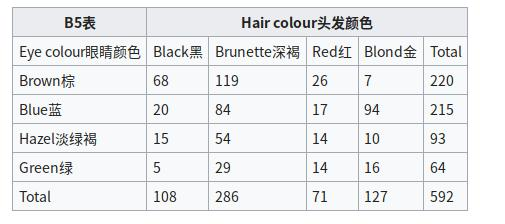
\includegraphics[width=10cm]{Screenshotfrom2022-01-18-5.jpg}

\textbf{实际(Obs.) vs 预计(Exp.)列联表 Contingency Table}:

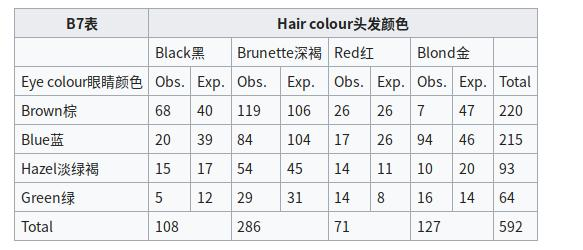
\includegraphics[width=10cm]{Screenshotfrom2022-01-18-6.jpg}

\hypertarget{ux9500ux552eux6570ux636eux591aux5143ux56deux5f52}{%
\subsubsection{销售数据------多元回归}\label{ux9500ux552eux6570ux636eux591aux5143ux56deux5f52}}

表C.1显示了某原料六年来的销售额、每吨平均价格和广告支出的情况。找出销售额与单价、广告费之间的回归关系,并评价这些回归方程式。这些方程式能否表达价格水平和广告支出对销售的影响?你能想出另一种总结数据的方法吗?

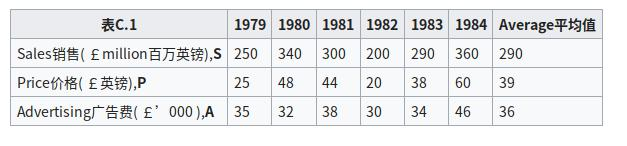
\includegraphics[width=10cm]{Screenshotfrom2022-01-18-7.jpg}

\hypertarget{ux4e8cux5143ux56deux5f52ux65b9ux7a0b}{%
\paragraph{二元回归方程}\label{ux4e8cux5143ux56deux5f52ux65b9ux7a0b}}

你可以立马使用统计分析工具,求出二元回归方程 {[}详见附件A4{]}:\\
S = 4.26P - 1.48A + 176 , R\textsuperscript{2} =0.955

你觉得这条回归方程式有用吗?没用。\\
首先不应该只用六个点来求一条二元回归方程,数据不够,所以我们更要了解这种回归方程式的局限:
这个例子也让我们可以看到两个相关因子产生的问题,例如:假设
P保持不变,增加 A, S应该会升,但以上的二元回归方程反而预测 S会下降。

所以-
1.48A(负数)不太合理,在二元回归中,因为因子之间相互影响,不能像单因子一元回归,可以这么简单地看参数正负。

应该怎么分析?\\
应从基本步骤开始, 当X Y都是连续数据,可先用散点图画出X Y之间的关系。对
S 和 P 也画散点图,看关系;然后 S 和 A ; P 与 A 之间也要看。
从这三个散点图可以看出S 和 P 有关系 A一直都比较稳定,但到最后一年,P和
A都升了很多 , S 也升。


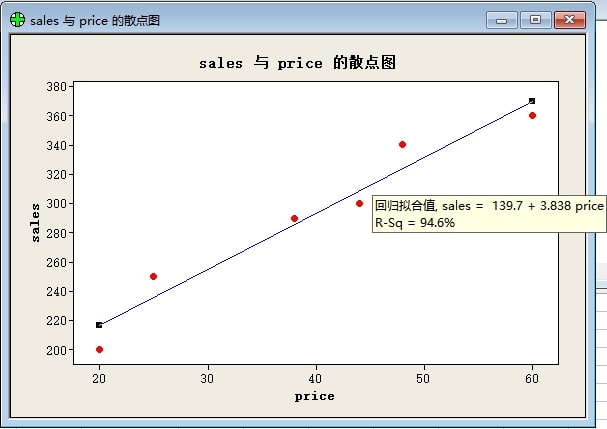
\includegraphics[width=10cm]{微信截图_20210702092718.jpg}\\

\hypertarget{ux4e00ux5143ux56deux5f52ux65b9ux7a0b}{%
\paragraph{一元回归方程}\label{ux4e00ux5143ux56deux5f52ux65b9ux7a0b}}

得出 S与P的线性关系方程式: S = 140 + 3.84 P , R\textsuperscript{2} =
0.946

(R\textsuperscript{2}越大代表这条线越能代表这些点,最高是1,代表这些点都在这条直线上面。)

同样对 S 与 A 做回归分析,但得出 R\textsuperscript{2} = 0.437
,表示关系较弱。所以就不用 A,只利用 P 求回归方程。

也可以 换个思路,用 V = S / P

得出 V与P的线性关系方程式:\\
V = 12.2 - 0.11 P , R\textsuperscript{2}=0.932


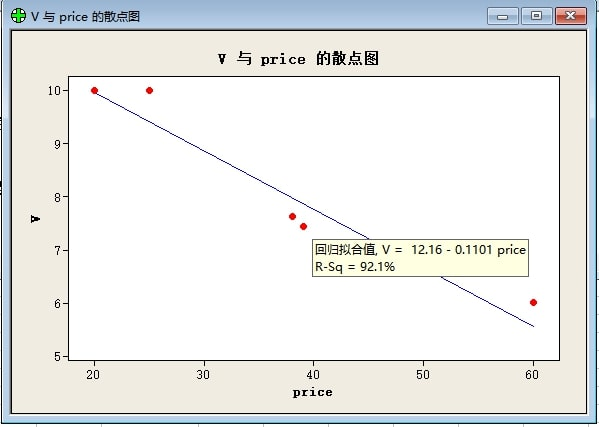
\includegraphics[width=10cm]{微信截图_20210702093001.jpg}\\

\hypertarget{ux56deux5f52ux5206ux6790ux7684ux6ce8ux610fux4e8bux9879}{%
\subsubsection{回归分析的注意事项}\label{ux56deux5f52ux5206ux6790ux7684ux6ce8ux610fux4e8bux9879}}

\framebox{%
\begin{minipage}[t]{0.97\columnwidth}\raggedright
注意:
我们可否利用以上回归方程来预测未来销售额?\\
不可以,尤其是如果广告预算有显著变化。
因我们计算回归方程时,没有利用广告费建模。(总共才六组数据也太少)\\
\textbf{问:}下一步应如何完善回归分析?\\
\textbf{答:}要先了解公司的广告预算策略, 例如,很多公司广告费是按销售的固定比例。
但也可能因为怕销售额下降,增加广告预算。了解后,便可以加入其他影响因素(如,广告),然后再多收集数据并分析。\strut
\end{minipage}}

其他注意事项:

\begin{itemize}
\tightlist
\item
  不能直接延伸,公式预测有适用范围
\item
  不应直接求公式,要先看看散点图关系
\end{itemize}

\hypertarget{ux76f4ux7ebfux5ef6ux4f38-extrapolation}{%
\subsubsection{直线延伸
Extrapolation}\label{ux76f4ux7ebfux5ef6ux4f38-extrapolation}}


\framebox{%
\begin{minipage}[t]{0.97\columnwidth}\raggedright
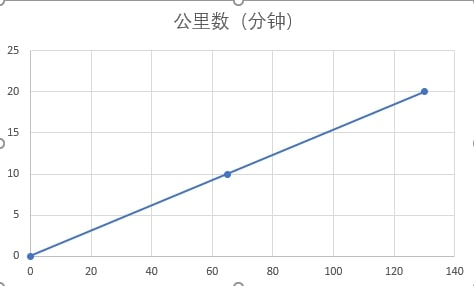
\includegraphics[width=10cm]{MarathonScreenshot_2021-04-17.jpg}\\
~\\
~\\
~\\
~\\
~\\
上图是某业余长跑手的统计,可以看到跑20公里用130分钟,形成一条直线(每6分半一公里),但我们不能利用这条直线推论他跑30公里的时间是10公里的3倍,甚至全马(40KM)时间是10公里的4倍。因为后期会因为体力不足而越来越慢。肯定不是一条直线,估计应是弧线,但弧度多少必须有他到40公里的数据才能得知。

那么以前的历史数据就没有什么用吗?
也不是,以往到20公里的数据可作为参考,只是不能简单当成直线延伸。\strut
\end{minipage}}

使用回归方程也一样,只能适用于有数据支持的范围。

\hypertarget{ux7ec4ux6570ux636eux7684ux56deux5f52ux65b9ux7a0b}{%
\subsubsection{4组数据的回归方程}\label{ux7ec4ux6570ux636eux7684ux56deux5f52ux65b9ux7a0b}}

\framebox{%
\begin{minipage}[t]{0.97\columnwidth}\raggedright
有下面四组XY,每组11对数据,回归方程(甚至X或Y的平均偏差)都一样,但是如果我们把每组数据生成散点图看,便看出,除了第一组数据,其他三组都不能用直线回归分析。\\

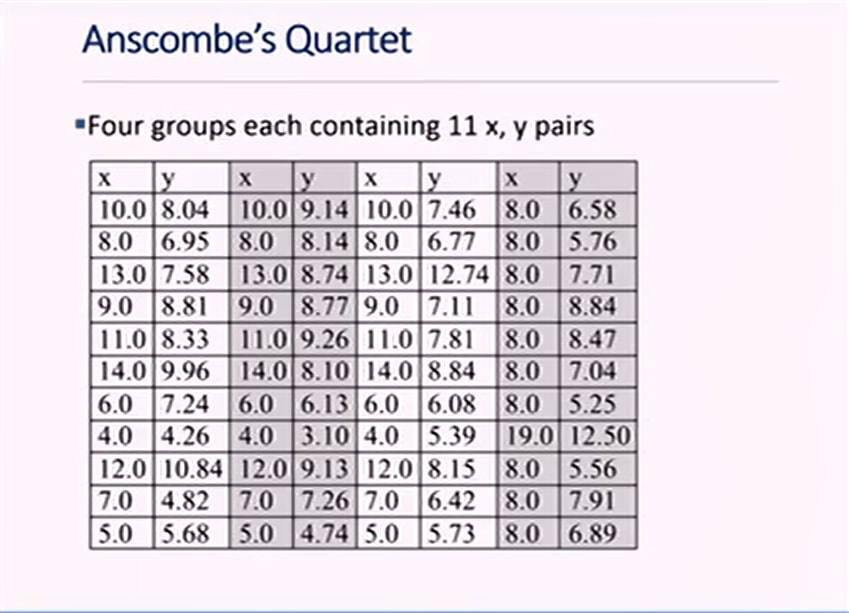
\includegraphics[width=6cm]{AnscombeQuartet1Screenshot_2021-04-07_215950.jpg}

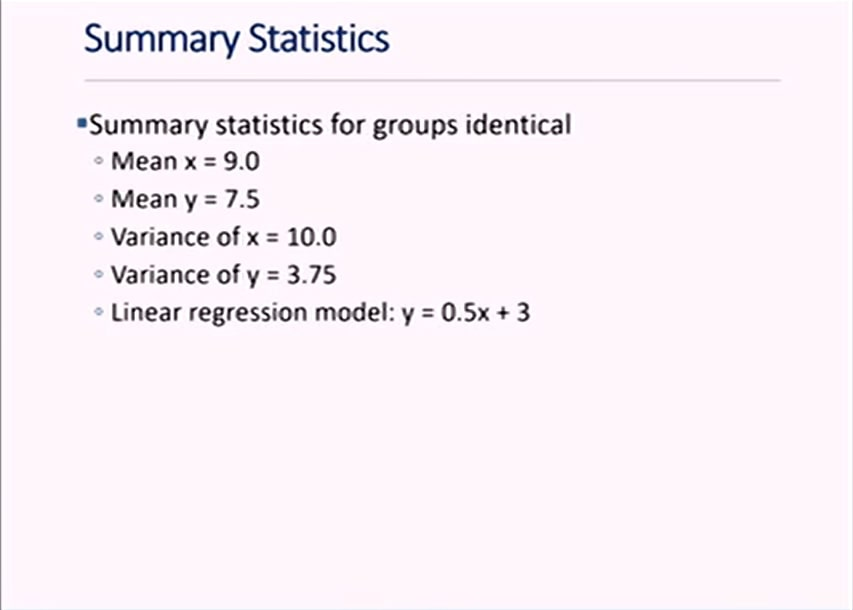
\includegraphics[width=10cm]{Quartet2Screenshot_2021-04-07_220127.jpg}

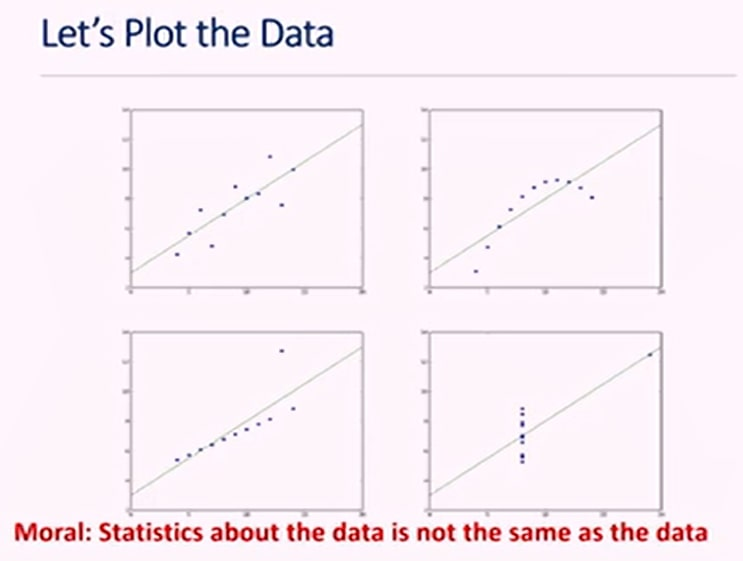
\includegraphics[width=10cm]{Quartet4Screenshot_2021-04-07_220427.jpg}

以上是1973年统计学家发表的例子,所以我们不应盲目地输入一堆数字,一键求出回归方程,便以为得出回归方程式和相关指数便完事,必需先画出数据的散点图,看看两个变量的关系。\strut
\end{minipage}}

\hypertarget{ux603bux7ed3}{%
\section{总结}\label{ux603bux7ed3}}

前部分主要讲如何描述数据:\\
统计分析主要是希望利用数据分析、统计方式帮我们解决问题(Problem
Solving)。所以题目叫MA(Measurement and
Analysis)度量与分析,度量本身的重点是如何分析,帮助解决问题。\\
度量与分析的重点其实与做问卷调查一样:\\
按目标策划收集那些数据?如何收集?如何分析?

数据分析员也应按以上思路, 才能更好地利用数据解决问题。

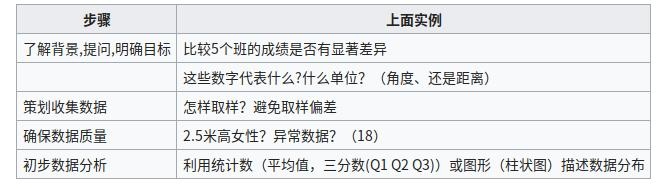
\includegraphics[width=10cm]{Screenshotfrom2022-01-18-8.jpg}

下半部主要介绍数据分析,与解读(Interpret) , 例如:

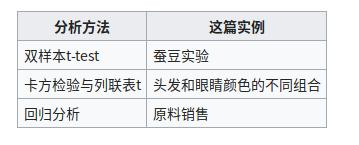
\includegraphics[width=10cm]{Screenshotfrom2022-01-18-9.jpg}

虽然计算机可以帮我们很快地分析数据,得出结论或者方程式,但也导致我们忽略了统计分析的根本:

\begin{itemize}
\tightlist
\item
  先了解问题与背景,明确目标
\item
  确保收集数据的质量
\item
  初步数据分析\\
\end{itemize}

所以在我们对两组蚕豆实验(有根,剪枝)数据做t-test之前,应该先看看两组数据的分布图。\\
做卡方检验之前更重要是先利用列联表 (Contingency
Table),看看眼色与发色之间有什么关系。\\
做回归分析之前, 必须先画散点图,看看两个变量之间的关系。\\
不要轻视数据分析前的描述性分析。

\hypertarget{ux5ea6ux91cfux7684ux76eeux7684ux662fux6c9fux901a}{%
\subsection{度量的目的是沟通}\label{ux5ea6ux91cfux7684ux76eeux7684ux662fux6c9fux901a}}

\framebox{%
\begin{minipage}[t]{0.97\columnwidth}\raggedright
与项目经理一起分析敏捷迭代数据:\\
十多年前,刚拿到六西格玛黑带,
我会首先把数据输入电脑、用工具分析,看数据之间有什么关系。

现在,当客户从6至8个敏捷迭代项目中,收集了6
-8轮数据,首先我问他们数据是如何收集?是否可靠?
然后会直接在白板上用水笔把各数据按每迭代,用不同颜色代表不同组,手画出每个项目的趋势,与他们项目经理一起讨论、判断,例如:数据范围是多少,是否稳定,需不需要细分......\\
因数据量少,完全不需要用统计分析工具,大家一起看白板讨论效果更好。\strut
\end{minipage}}

美国软件工程顾问Gerald M WEINBERG
先生说过,``如果你的数据分析需要超过初中程度的话,你要想想这种分析是否有效?''

在CMMI高成熟度咨询时,常常有人问:我们在CMMI不是要求高层也用统计分析来管理吗?如何实现?\\
我这样解读:公司要做到高成熟度,不可能要求每个员工,包括高层都是六西格玛黑带、统计学博士。可能有些详细的分析需要很多统计的技巧,但是分析员最终要用一些每位干系人(包括老板,项目经理,团队成员)都听得懂的方式把那些结果分析出来,让他看得懂。但我看很多公司的统计分析员,只是沉迷于大数据,深度学习、AI等``高级''方法,以为无论什么数据,都可以使用统计分析,得出X-Y的关系方程式,反而忽略了一些基本道理:\\
\textbf{如果你可以把你的分析结果跟你的孩子说得清,这种统计分析才算有效。}\\

\hypertarget{appendix-ux9644ux4ef6}{%
\section{Appendix 附件}\label{appendix-ux9644ux4ef6}}

\hypertarget{a-ux5982ux4f55ux753bux830eux53f6ux56festem-and-leaf-plot}{%
\subsection{A: 如何画茎叶图(Stem and leaf
plot)}\label{a-ux5982ux4f55ux753bux830eux53f6ux56festem-and-leaf-plot}}

以文中20名学生在数学考试分数为例:

\begin{enumerate}
\tightlist
\item
  把分数从小到大排序
\item
  从上而下画一直线
\item
  第一个数 30 , 左边写 3 , 右面写 0 (叶)
\item
  排第二是 35 , 因5大于 0 - 4, 新一行,左边写 3 , 右面写 5 (叶)
\item
  37, 因7 属于 5 - 9 , 所以同一行 , 在 5 右面写 7 (叶)
\item
  最终便可以简单利用数目字形成一个横放的直方图
\end{enumerate}

\hypertarget{a-ux7bb1ux7ebfux56fe-box-and-whisker-plot}{%
\subsection{A: 箱线图 (Box and Whisker
Plot)}\label{a-ux7bb1ux7ebfux56fe-box-and-whisker-plot}}


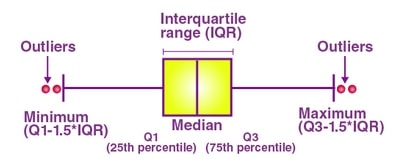
\includegraphics[width=10cm]{BoxWhiskerScreenshot_2021-08-02_214603.jpg}

箱线图包括5个数:

\begin{itemize}
\tightlist
\item
  Minimum 最少 (Q0 )
\item
  1st Quartile (Q1 , 25 percentile) 箱子的左面边线
\item
  Medium 中位数 (Q2 , 50 percentile) 箱子中间的线
\item
  3rd Quartile (Q3 , 75 percentile) 箱子的右面边线
\item
  Maximum 最大 (Q4 , 100 percentile)
\end{itemize}

有些箱线图直接把两头指到最大与最少,不展示离散点 (outliers)。

Interquartile range (IQR) = Q3 - Q1

\hypertarget{a-2-sample-t-test}{%
\subsection{A: 2-sample T test}\label{a-2-sample-t-test}}

\hypertarget{ux4f8bux5927ux5b66ux4f53ux80b2ux6d3bux52a8}{%
\subsubsection{例:大学体育活动}\label{ux4f8bux5927ux5b66ux4f53ux80b2ux6d3bux52a8}}

假设:大学为男生提供的运动项目的平均数量大于为女生提供的,下面是随机抽样美国各大学为男女生提供的体育项目量,如果Alpha*=0.10,检验男女是否有显著差别。(假定,男女生数据的标准差都一样
δ1=δ2 = 3.3)

\texttt{~*~Alpha(显著性水平)~是指当零假定是真,但被拒绝的错误率。(也称为第I类错误)~}\\
\texttt{~置信区间(Confidence~interval)~=~1~-~alpha}


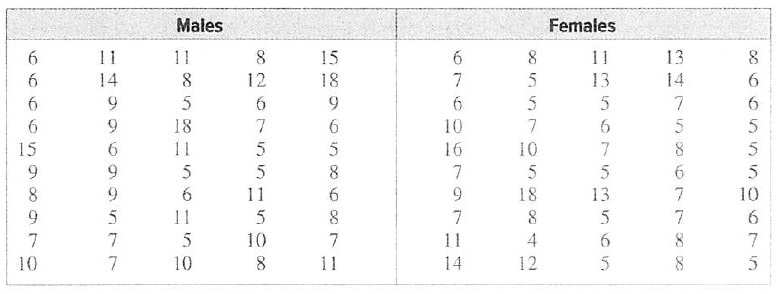
\includegraphics[width=10cm]{男女生.jpg}

\hypertarget{minitab}{%
\paragraph{Minitab}\label{minitab}}

检验两个独立样本平均值之间是否有显著差异\\
零假设 - 两者没有显著差异

先看看两组的柱状图 (minitab):


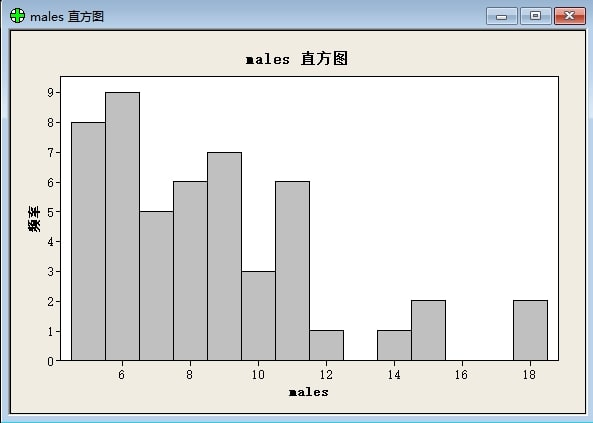
\includegraphics[width=10cm]{微信截图_20210615141207.jpg}


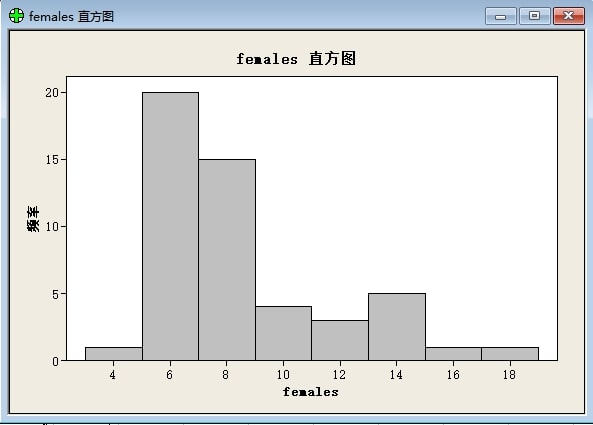
\includegraphics[width=10cm]{微信截图_20210615141235.jpg}

\begin{enumerate}
\tightlist
\item
  统计-基本统计量-双样本T(2)
\end{enumerate}

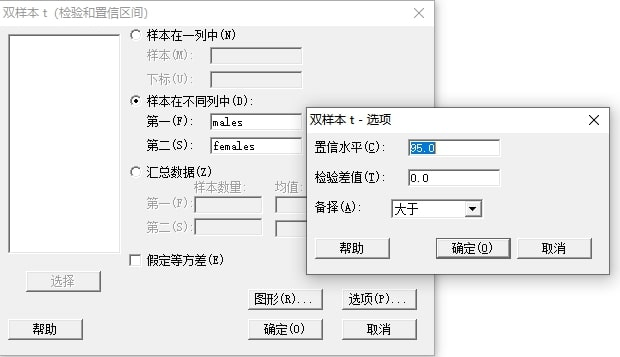
\includegraphics[width=10cm]{微信截图_20210615142847.jpg}


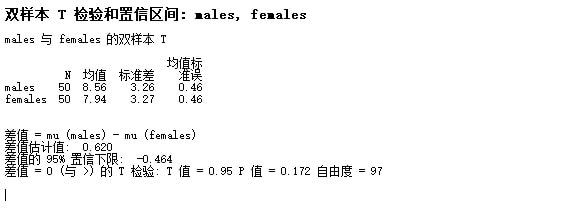
\includegraphics[width=10cm]{微信截图_20210615142815.jpg}

由于p值大于显著性水平,0.172\textgreater{} 0.05,所以不能拒绝零假设 -
两者没有显著差异。

\hypertarget{a-anova}{%
\subsection{A: ANOVA}\label{a-anova}}

\hypertarget{ux793aux4f8b12-1ux6bcfux52a0ux4ed1ux6c7dux6cb9ux884cux9a76}{%
\subsubsection{示例12-1每加仑汽油行驶}\label{ux793aux4f8b12-1ux6bcfux52a0ux4ed1ux6c7dux6cb9ux884cux9a76}}

研究人员想看看三种不同类型的汽车:小型汽车(small)、轿车(sedans)和豪华汽车(luxury)在城市驾驶时的燃油经济性是否有差异。他随机抽样了四种小型汽车、五种轿车和三种豪华汽车。每加仑的英里数都都在下面列出。在α=
0.05时,检验三种平均值之间是否没有显著差异。{[}Source: US Environmental
Protection Agency{]}

\hypertarget{anova-ux4f8bux5b50}{%
\paragraph{ANOVA 例子}\label{anova-ux4f8bux5b50}}

1:零假设:三种不同类型的汽车:小型汽车、轿车和豪华汽车在城市驾驶时的燃油经济性平均值之间没有差异\\
2:也可用统计工具 Minitab 做 ANOVA分析,并算出P值=0.038 低于0.05
,所以拒绝零假设, 三类有显著差异\\

\hypertarget{minitab-1}{%
\subsubsection{minitab}\label{minitab-1}}


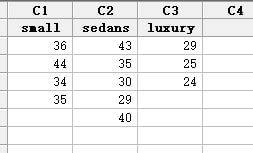
\includegraphics[width=10cm]{微信截图_20210709102603.jpg}

统计-方差分析-单因子(未堆叠存放)


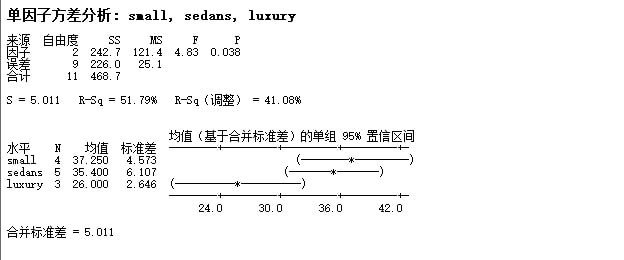
\includegraphics[width=10cm]{微信截图_20210709102700.jpg}

\hypertarget{a-ux5361ux65b9ux68c0ux9a8cux4e0eux5217ux8054ux8868-contingency-table}{%
\subsection{A: 卡方检验与列联表 Contingency
table}\label{a-ux5361ux65b9ux68c0ux9a8cux4e0eux5217ux8054ux8868-contingency-table}}

一位研究人员希望了解医院和病人感染的数量之间是否有关系。我们随机抽取了3家医院,并报告了特定年份的感染人数。数据如下。

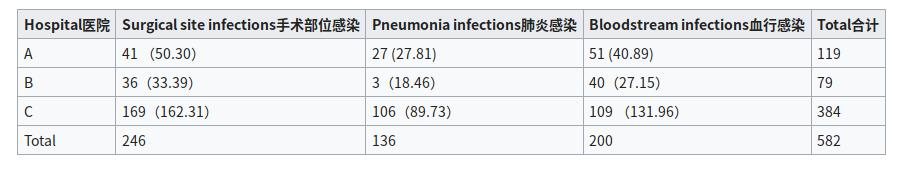
\includegraphics[width=10cm]{Screenshotfrom2022-01-18-10.jpg}

\hypertarget{ux5361ux65b9ux68c0ux9a8cux4f8bux5b50}{%
\paragraph{卡方检验例子}\label{ux5361ux65b9ux68c0ux9a8cux4f8bux5b50}}

1:零假设:医院(Hospitals) 与 感染种类(Infections) 之间没有相关

2:Degree of
Freedom(DF)=(3-1)×(3-1)=4,从卡方参考列表,α=0.05对应的卡方关键值是9.488

3:首先使用以下公式计算每个列联表的预计值E(Expected
Value),得出E写在()中


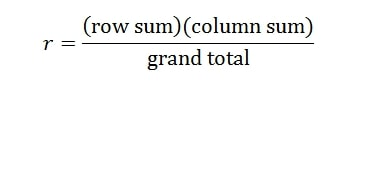
\includegraphics[width=10cm]{公式卡方1.jpg}

%\(E = \frac{(\mbox{行 总 数}\ row\sum) * (\mbox{栋 总 数}\ column\sum)} {\mbox{所 有 总 数}\ grand\total}\)

%<math> E = \frac{(\mbox{行 总 数}\ row\sum) * (\mbox{栋 总 数}\ column\sum)} {\mbox{所 有 总 数}\ grand\total} </math> 

再用下面公式从预计值与实际值O(Observed value),计算卡方值 :

\href{文件:卡方公式2Screenshot_2021-09-24_121105.jpg}{文件:卡方公式2Screenshot
2021-09-24 121105.jpg}

%\(\chi ^2 = \sum \frac{(O - E)^2} {E}\)

%<math> \chi ^2 = \sum \frac{(O - E)^2} {E}</math> 

4:得出卡方=30.7
,比预估关键值(9.488)高,所以拒绝零假设,医院(Hospitals) 与
感染种类(Infections) 之间相关\\
也可用统计工具 Minitab 得出卡方,算出P值低于0.05 ,所以拒绝零假设 :\\
统计-表格-卡方检验(工作表中双向表)


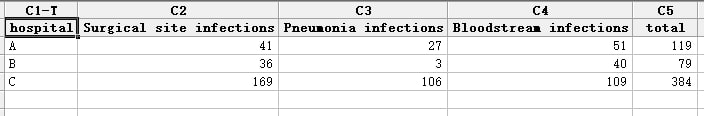
\includegraphics[width=10cm]{微信截图_20210708092203.jpg}


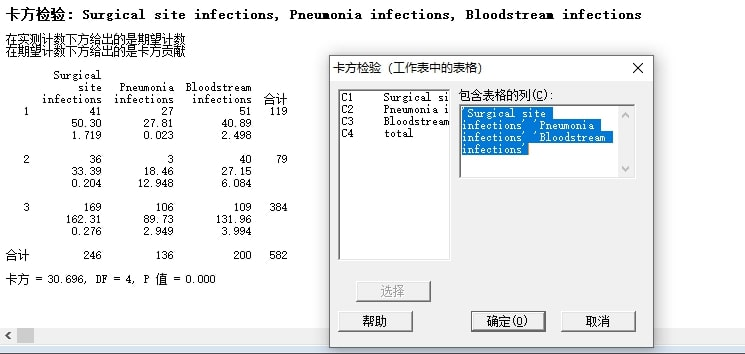
\includegraphics[width=10cm]{微信截图_20210708094035.jpg}

\hypertarget{a-linear-regression}{%
\subsection{A: Linear Regression}\label{a-linear-regression}}

回归分析希望找出一条直线,它与每个点的距离的平方总和最小。


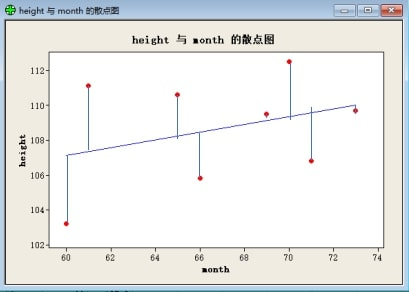
\includegraphics[width=10cm]{微信截图_20210702093730.jpg}

\hypertarget{ux8be5ux5982ux4f55ux505aux56deux5f52ux5206ux6790}{%
\subsubsection{该如何做回归分析?}\label{ux8be5ux5982ux4f55ux505aux56deux5f52ux5206ux6790}}

\begin{itemize}
\tightlist
\item
  如果使用电脑程序,通过``最小二乘法''计算并绘制这条线。
\end{itemize}


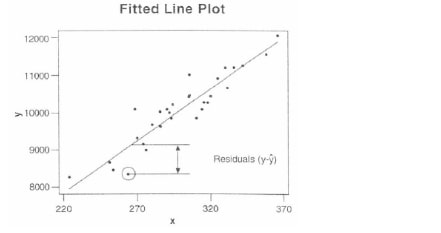
\includegraphics[width=10cm]{微信截图_20210702093859.jpg}

\begin{enumerate}
\tightlist
\item
  计算相关系数R,使用下面的方程式。
\item
  通过使用方程式y=mx+b,确定斜率或线的y轴截距。
\end{enumerate}

\begin{itemize}
\tightlist
\item
  y截距是``最佳拟合线''穿过的在y轴上的点(在这一点,x=0)。
\item
  线的斜率(m)按照y的变化除以x的变化来计算(m=∆y/∆x)。斜率m也认作预测变量x的系数。
\item
  R\textsuperscript{2}
  衡量回归方程能多好代表这些点,最理想状态,R\textsuperscript{2}
  等于1,表示零误差,所有的点都在回归线上。
\end{itemize}

\hypertarget{ux4f8b10-1ux6c7dux8f66ux79dfux8d41ux516cux53f8}{%
\subsubsection{例10-1汽车租赁公司}\label{ux4f8b10-1ux6c7dux8f66ux79dfux8d41ux516cux53f8}}

以下为美国随机抽样六家汽车租赁公司最近一年的总收入(亿美元)。


\includegraphics[width=10cm]{表10-1.jpg}

\hypertarget{ux89e3ux51b3ux65b9ux6cd5}{%
\subsubsection{解决方法}\label{ux89e3ux51b3ux65b9ux6cd5}}

\begin{itemize}
\tightlist
\item
  绘制散点图,如图10-2所示
\end{itemize}

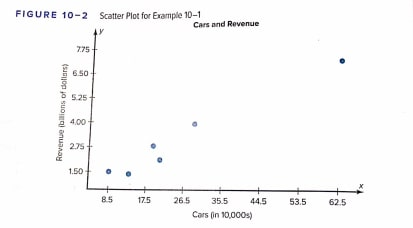
\includegraphics[width=10cm]{微信截图_20210630161521.jpg}

\begin{itemize}
\tightlist
\item
  确定是否存在关系。发现代理商拥有的汽车数量和公司的总收入之间似乎存在正线性关系。
\end{itemize}


\includegraphics[width=10cm]{表10-4_2.jpg}

\begin{itemize}
\tightlist
\item
  代入公式,计算出R
\end{itemize}


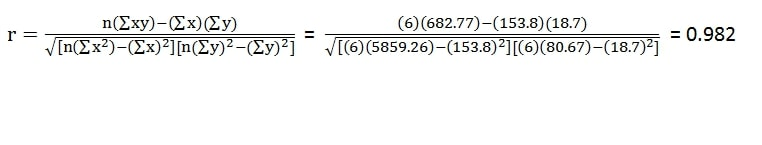
\includegraphics[width=10cm]{公式10-1.jpg}

结论:汽车租赁公司的汽车数量和它的年销售额之间有很强的正相关关系,也就是说,汽车租赁公司拥有的汽车越多,公司的年销售额就越多

\hypertarget{ux4e5fux53efux4ee5ux7528-minitab}{%
\subsubsection{也可以用
minitab}\label{ux4e5fux53efux4ee5ux7528-minitab}}


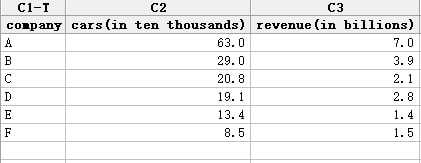
\includegraphics[width=10cm]{微信截图_20210709103157.jpg}

图形-散点图(回归分析)


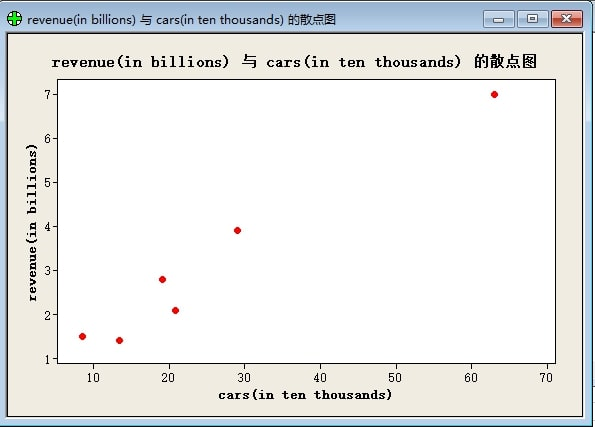
\includegraphics[width=10cm]{微信截图_20210709103117.jpg}


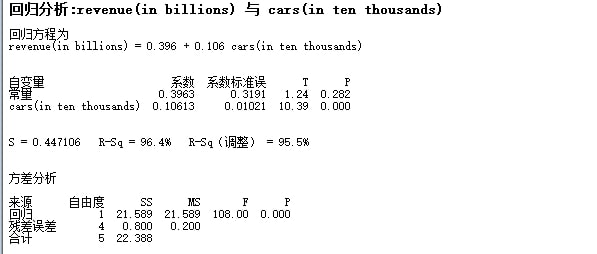
\includegraphics[width=10cm]{微信截图_20210709103241.jpg}

也得出 R\textsuperscript{2} = 96.4\% , 调整后 = 95.5\%\\
Revenue (年销售额) = 0.396 + 0.106 x Cars (汽车数量)\\

\cite{MA1References1}
\cite{MA1References2}
\cite{MA1References3}

